\section{问题一：无泄漏观看人数预测}

\subsection{数据边界与特征构造}

目标是在开球前预测转播观看人数。附件 $15$ 张表共 $2241$ 行，其中历史比赛表提供 $560$ 条训练记录和 $140$ 条时间外测试记录，另有 $72$ 场模拟小组赛需要预测。记录按比赛日期和编号稳定排序；同场进球、xG、射门、控球、上座与观看人数不作直接特征，只把严格早于开球日期的球队记录汇总为最近 $5$ 场均值和半衰期 $5$ 场的指数加权均值。同一日期的比赛先生成特征，日末再统一更新历史。

每个外层时间折都独立完成缺失值填补、类别编码、标准化和模型拟合。最早外折的训练窗内部完成一次超参数选择，此后冻结参数并在五个外折上重拟合；验证窗的观看标签在历史特征重建前整段置空。最终生产特征共 $55$ 列，其中 $10$ 个同场赛后字段被禁止直接进入模型，中立场标记因解释贡献有限而舍弃。未来 $72$ 场使用统一的赛前快照，不调用问题二尚未确定的场馆和时段。

对比赛 $j$，双方某项实力量 $E$ 写成均值与绝对差：
\begin{equation}
E_j^{\mathrm{mean}}=\frac{E_{ja}+E_{jb}}{2},\qquad
E_j^{\mathrm{gap}}=|E_{ja}-E_{jb}|.
\end{equation}
赔率先去除水位，再计算三种赛果概率的熵：
\begin{equation}
\pi_{jc}=\frac{o_{jc}^{-1}}{\sum_k o_{jk}^{-1}},\qquad
H_j^{\mathrm{odds}}=-\sum_{c\in\{a,D,b\}}\pi_{jc}\log\pi_{jc}.
\end{equation}
任一特征的最晚来源时刻都必须早于开球时刻；赛事阶段、时区和预先指定交互只作条件预测量，不作因果解释。

\subsection{样本分布与候选模型}

表\ref{tab:q1-descriptive}给出核心变量尺度。训练集观看人数均值为 $145.64$ 百万人，中位数为 $142.11$ 百万人，四分位区间为 $[128.43,160.62]$；最大值 $225.41$ 百万人使分布呈右尾。图\ref{fig:q1-target-raincloud}显示密度峰约在 $140$ 百万人，右尾连续延伸，并非少数孤立异常值。故本文保留高观看样本，不对目标截断；MSE 选模会放大尾部误差，后续用时间外残差单独描述其不确定性。

\begin{table}[H]
\centering
\caption{问题一核心变量描述性统计}
\label{tab:q1-descriptive}
\small
\resizebox{\textwidth}{!}{%
\begin{tabular}{lrrrrrrrr}
\toprule
变量 & 样本数 & 均值 & 标准差 & 最小值 & P25 & 中位数 & P75 & 最大值 \\
\midrule
观看人数 & 560 & 145.64 & 23.56 & 93.96 & 128.43 & 142.11 & 160.62 & 225.41 \\
平均Elo & 560 & 1756.86 & 120.58 & 1472.50 & 1671.00 & 1758.00 & 1846.50 & 2025.50 \\
平均排名 & 560 & 24.30 & 9.97 & 2.50 & 17.00 & 24.00 & 31.50 & 47.50 \\
平均球迷基础 & 560 & 73.41 & 10.47 & 46.30 & 66.05 & 73.03 & 81.93 & 94.40 \\
赔率熵 & 560 & 1.00 & 0.10 & 0.71 & 0.95 & 1.04 & 1.08 & 1.10 \\
\bottomrule
\end{tabular}
}
\vspace{2pt}
\noindent\begin{minipage}{0.96\textwidth}\footnotesize 注：观看人数单位为百万人；其余变量采用源数据或赛前构造口径。\end{minipage}
\end{table}


\begin{figure}[htbp]
\centering
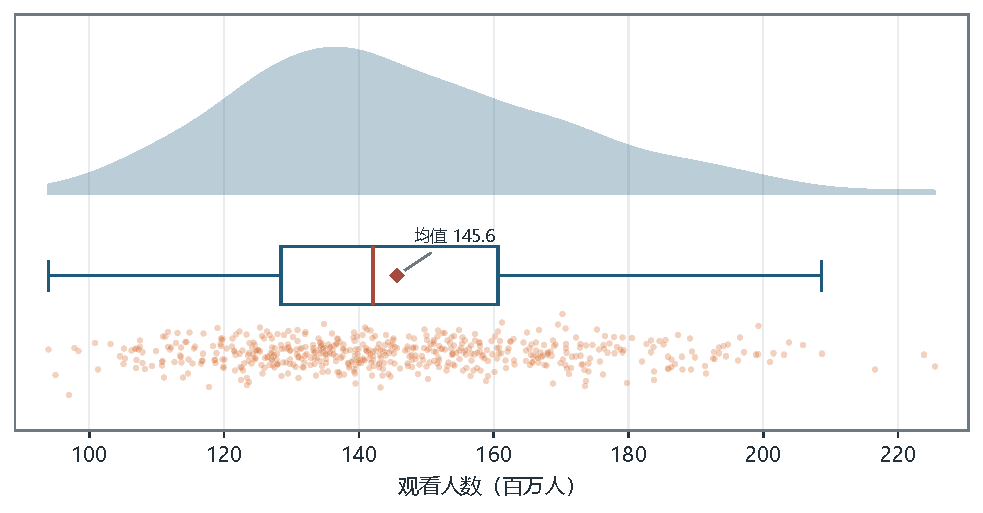
\includegraphics[width=0.72\textwidth,height=0.22\textheight,keepaspectratio]{../figures/fig_q1_target_raincloud.pdf}
\caption{训练集观看人数分布与右尾特征}
\label{fig:q1-target-raincloud}
\end{figure}

平均 Elo、平均排名、平均球迷基础与观看人数的线性相关系数约为 $0.62$、$-0.61$ 和 $0.69$，赔率熵约为 $0.31$。平均 Elo 与平均排名高度反向，特征之间存在明显共线；同一实力区间内的观看人数仍较分散，单变量也不足以解释需求。候选模型因此包括均值基线、Elastic Net、ExtraTrees 和 CatBoost，用同一时间折比较线性正则化与非线性机制。

Elastic Net 的估计量为
\begin{equation}
\widehat\beta=\arg\min_\beta\left\{
\frac{1}{n}\sum_{j=1}^{n}(Y_j-X_j^\top\beta)^2+
\alpha\left[\rho\lVert\beta\rVert_1+
\frac{1-\rho}{2}\lVert\beta\rVert_2^2\right]\right\}.
\end{equation}
网格取 $\alpha\in\{10^{-3},10^{-2},10^{-1},1,10\}$、$\rho\in\{0.1,0.5,0.9\}$，最终选择 $\alpha=1.0,\rho=0.9$。ExtraTrees 固定 $600$ 棵树并比较叶节点下限与特征比例；CatBoost 最多训练 $3000$ 轮，在折内末 $20\%$ 时间段早停。

\subsection{时间外验证与模型选择}

表\ref{tab:q1-model-summary-short}显示，Elastic Net 的平均 MSE 为 $220.086$，低于 CatBoost 的 $234.209$ 和 ExtraTrees 的 $250.162$；相对均值基线 $581.203$，MSE 降低约 $62.1\%$。RMSE 与 MAE 给出同一排序，说明选模结果不依赖单一损失口径。五折逐折误差及其稳定性在第\ref{sec:sensitivity}节继续检验。

\begin{table}[htbp]
\centering
\caption{候选模型时间外误差汇总}
\label{tab:q1-model-summary-short}
\begin{tabular}{lrrr}
\toprule
模型 & 平均 MSE & 平均 RMSE & 平均 MAE \\
\midrule
Elastic Net & 220.086 & 14.812 & 11.828 \\
CatBoost & 234.209 & 15.267 & 12.184 \\
ExtraTrees & 250.162 & 15.778 & 12.734 \\
均值基线 & 581.203 & 24.099 & 19.333 \\
\bottomrule
\end{tabular}
\end{table}

复杂模型没有抵消小样本方差：CatBoost 与 ExtraTrees 的 MSE 分别高出 $15.967$ 和 $30.076$。因此按预先规定的规则选择 Elastic Net，在全部 $560$ 条训练样本上重拟合，并保留 $465$ 条时间外 OOF 预测用于区间和残差分析。

\subsection{诊断、解释与预测输出}

OOF 拟合见图\ref{fig:q1-prediction-fit}。整体 $R^2$ 约为 $0.620$、RMSE 约为 $14.84$ 百万人；真实值超过约 $190$ 百万人后，预测更常落在 $45$ 度线下方，表明正则化模型对高关注赛事存在收缩性低估。残差均值为 $-0.00093$ 百万人，日期序列在 $2019$--$2024$ 年间围绕零线波动，没有持续同向漂移；Q--Q 尾部的轻微偏离说明经验区间比正态近似更合适。

\begin{figure}[htbp]
\centering
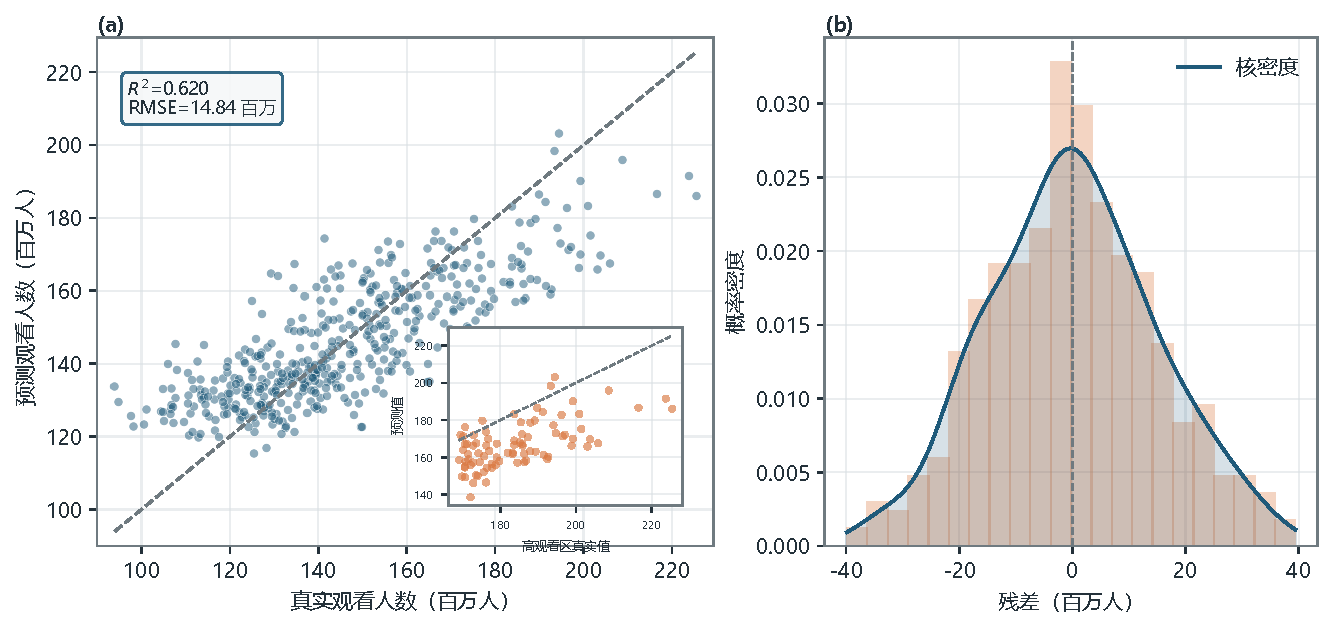
\includegraphics[width=0.80\textwidth,height=0.48\textheight,keepaspectratio]{../figures/fig_q1_prediction_fit.pdf}
\caption{最终模型 OOF 预测拟合与残差分布}
\label{fig:q1-prediction-fit}
\end{figure}

OOF 残差的 $5\%$ 与 $95\%$ 分位数分别为 $-22.7075$ 和 $25.1737$ 百万人。对点预测 $\widehat Y(x)$，本文使用
\begin{equation}
PI_{0.90}(x)=\left[\max\{0,\widehat Y(x)-22.7075\},\ \widehat Y(x)+25.1737\right]
\end{equation}
描述历史时间外误差；它不是严格的条件置信区间。

图\ref{fig:q1-shap-summary}给出后 $20\%$ 验证窗口的置换重要性和单样本影响。打乱平均球迷基础后 MSE 增加 $238.032$，高于世界杯标记 $32.597$、球迷基础--世界杯交互 $26.379$ 和实力--赔率熵交互 $24.145$。主要信号集中在少数连续特征及预先指定交互，解释了线性正则化为何优于当前非线性候选；这些数值只表示预测贡献，不表示因果效应。

\begin{figure}[htbp]
\centering
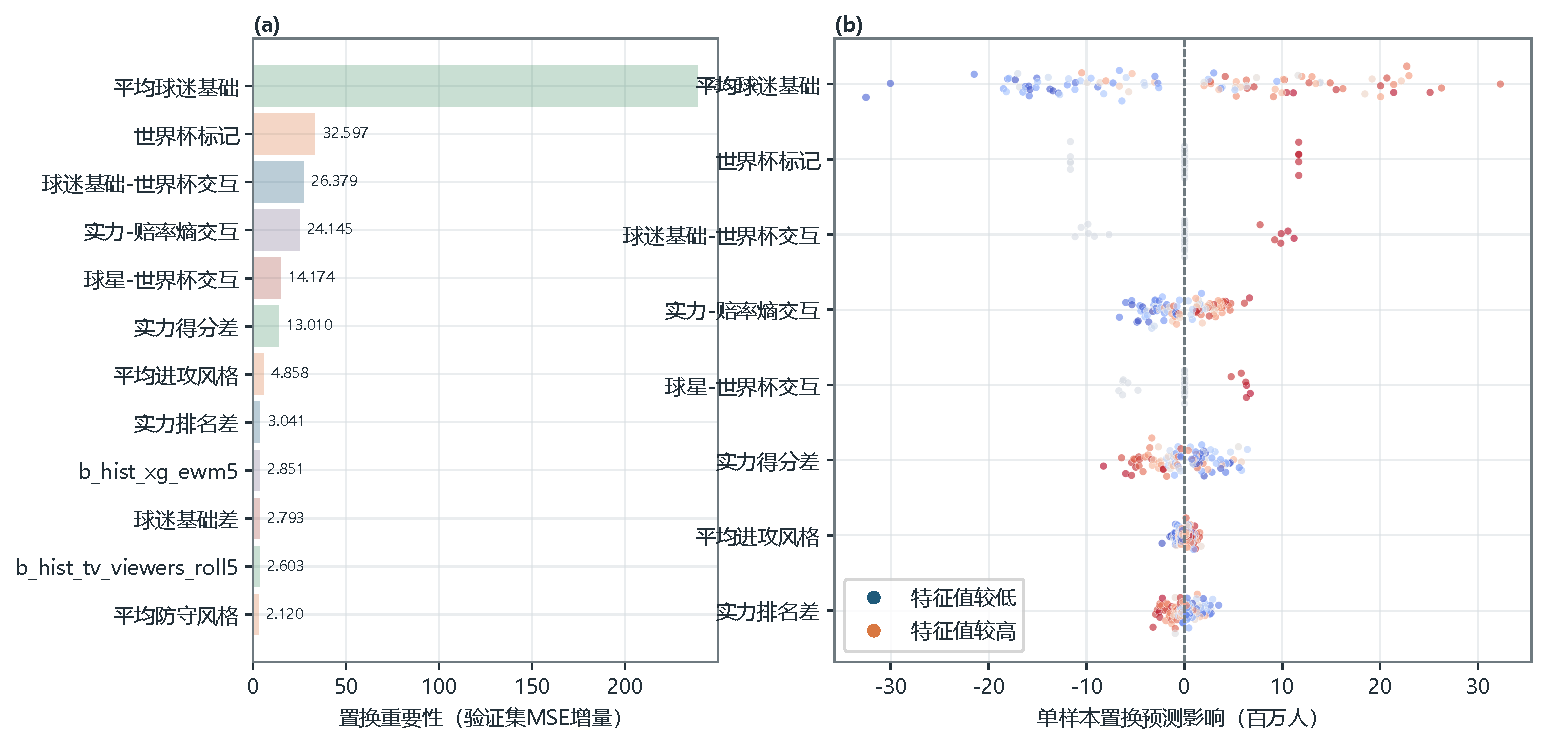
\includegraphics[width=0.82\textwidth,height=0.30\textheight,keepaspectratio]{../figures/fig_q1_shap_summary.pdf}
\caption{Elastic Net 置换重要性与单样本预测影响}
\label{fig:q1-shap-summary}
\end{figure}

最终模型对 $140$ 条测试记录的预测范围为 $115.783$--$188.216$ 百万人，均值 $145.331$ 百万人，均为有限正值。$72$ 场模拟小组赛的预测范围为 $144154622$--$205695590$ 人，均值 $170321280$ 人；两份结果保持模板主键、行数和单位。问题二只接收这 $72$ 场赛前点预测，不读取测试标签或赛后字段。
